\chapter{Odporna optymalizacja w~sąsiedztwie}\label{ch:localSearch}
\thispagestyle{chapterBeginStyle}





Posiadamy już wszystkie potrzebne nam narzędzia, aby móc pochylić się nad głównym problemem, który interesował nas od samego początku, a~który wymagał od nas stopniowego wprowadzania coraz to bardziej złożonych instancji problemów: od problemu minimalnego drzewa rozpinającego, przez problemy: \textsc{IMST}, \textsc{AIMST}, aż po problem odpornej optymalizacji z~możliwością poprawy rozwiązania, którym to zajmiemy się w~poniższym rozdziale.
Nim jednak to nastąpi, będziemy chcieli krótko podsumować dotychczas zebrane informacje, by później przejść do opisu, wspomnianych już wcześniej, algorytmów lokalnego przeszukiwania dla problemu \textsc{RRIMST}.
Jedną z~podstawowych i~bardzo wydajnych metod konstrukcji rozwiązań problemów optymalizacyjnych jest metoda oparta na przeszukiwaniu bezpośrednich \textbf{sąsiadów} aktualnie posiadanego rozwiązania z~nadzieją, że takie krokowe zachowanie się algorytmu będzie skutkowało szybkim zbliżaniem się do optymalnego rozwiązania.
W~poniższym rozdziale wskażemy trzy takie metody, przy czym jedną z~nich~--- tą najefektywniejszą~--- omówimy bardziej szczegółowo.
Choć wydawać by się mogło, że taka metoda rozwiązywania problemów optymalizacyjnych nie ma prawa się dobrze zachowywać (ze względu na bardzo silne założenia dotyczące sposobu zachowywania się rozwiązań sąsiednich względem obecnie badanego), to właśnie takie algorytmy~--- szczególnie \textbf{Tabu Search}~--- są najogólniejszym sposobem na rozwiązywanie problemów optymalizacyjnych.




\section{Odporna optymalizacja z~możliwością poprawy}




Tak jak to wielokrotnie przytaczaliśmy, matematyczny opis problemu \textsc{Recoverable Robust Incremental Minimum Spanning Tree} składa się z~wielu, dotychczas przez nas omówionych, komponentów,~a~u którego podstaw leży, przedstawiony w~rozdziale \ref{ch:mst}, problem minimalnego drzewa rozpinającego dla grafu $G = \left( V, E \right)$.
Następnym naszym krokiem było zwrócenie uwagi na nieco bardziej złożony problem przyrostowy dla grafu $G$, gdzie ograniczaliśmy się do poszukiwań takich rozwiązań, które nie różniły się w~znaczący sposób od początkowego rozwiązania, które wybieraliśmy na samym początku. 
Założyliśmy wtedy, iż takim scenariuszem, dla którego wybieraliśmy wspomniane rozwiązanie, będzie scenariusz $\textbf{s}_{0}$, i~że to od minimalnego drzewa rozpinającego $T^{\ast}_{\textbf{s}_{0}}$ będzie zależeć rozwiązanie problemu \textsc{IMST}, wybierane na podstawie następnych scenariuszy, oryginalnego rozwiązania $T^{\ast}_{\textbf{s}_{0}}$ oraz parametru $k$, który określa jak wiele krawędzi może zawierać nowe rozwiązanie, których $T^{\ast}_{\textbf{s}_{0}}$ nie zawiera.
Następnym naszym krokiem było przedstawienie schematu konstrukcji rozwiązania dla problemu adwersarza (patrz rozdział \ref{ch:minmax}) z~dyskretnym zbiorem scenariuszy $S = \left\{ \textbf{s}_{1}, \textbf{s}_{2}, \dots, \textbf{s}_{l} \right\}$, gdzie zadaniem adwersarza było wybranie takiego scenariusza, z~dostępnego dla niego zbioru $S$, aby najbardziej korzystne rozwiązanie problemu minimalnego drzewa rozpinającego w~wersji \textsc{Incremental} ze scenariuszem początkowym $\textbf{s}_{0}$ było jak najgorsze (z~jego perspektywy jak najlepsze).
Ustaliliśmy, że dzięki specyficznej definicji tego problemu, istnieje możliwość jego błyskawicznego rozwiązania (dzięki możliwości podzielenia zadań na osobne wątki procesora), w~czasie niewiele większym niż ten, który jest wymagany dla wcześniej wspomnianego problemu \textsc{IMST}, którego rozwiązanie potrafiliśmy znaleźć w~czasie wielomianowym (sposób, w~jaki to robiliśmy, przedstawiony został w~rozdziale \ref{ch:binaryIncMST}).
Następnym naszym krokiem będzie budowa algorytmu, który umożliwi nam poradzenie sobie z~problemem, którego matematyczny opis przypominamy w~równaniu \ref{eq:rrimst}~--- jak zostało pokazane, problem ten jest już na tyle złożony, że nie tylko jest \textsc{NP}-trudny, lecz nie jest on w~żaden sposób aproksymowalny~\cite[twierdzenie $6$]{Kasperski2014}.
Oznacza to, że nie istnieje algorytm, gdzie zwracane przez niego rozwiązania moglibyśmy traktować jako te co najwyżej $p$ razy gorsze od rozwiązania optymalnego (tak jak to miało miejsce w~przypadku problemu \textsc{Min-Max} dla dyskretnych zbiorów scenariuszy~--- zobacz twierdzenia: \ref{th:minmaxavg} i~\ref{th:minmaxworst}).
W~związku z~tym musimy znaleźć inny sposób na radzenie sobie z~postawionym przed nami problemem.




\section{Algorytm zachłanny}




\textbf{Algorytm zachłanny} jest najbardziej podstawową i~naturalną strategią poszukiwania rozwiązania dla problemów optymalizacyjnych w~myśl zasady ,,jeśli wartość mojego rozwiązania jest niewiele gorsza od wartości optymalnej, za pomocą niewielkich zmian powinienem tą wartość osiągnąć''.
Fundament, na którym zbudowane jest to zdanie, zawiera bardzo ważne założenie, określające charakter zachowania się poszczególnych rozwiązań problemu optymalizacyjnego.
Zakładamy bowiem, że proporcjonalnie do wielkości zmian wprowadzonych w~znalezionym rozwiązaniu, rośnie (bądź maleje) koszt takiego rozwiązania.
Takim problemem jest na przykład rozpatrywane przez nas zagadnienie minimalnego drzewa rozpinającego, który leży u~podstaw problemu, na którego rozwiązanie poświęcimy cały poniższy rozdział:

\begin{equation}\label{eq:rrimst}
	\min_{\mathclap{\textbf{x} \in X}} \left( v \left( \textbf{x}, \textbf{s} \right) + \max_{\mathclap{\textbf{s}^{\prime} \in S}} \min_{\mathclap{\textbf{y} \in X^{k}_{\textbf{x}}}} v \left( \textbf{y}, \textbf{s}^{\prime} \right) \right)\text{.}
\end{equation}



\subsection{Sąsiedztwo}



Rozpoczniemy wyjątkowo od przedstawienia pseudokodu algorytmu zachłannego (zobacz pseudokod \ref{alg:localsearch})\footnote{
	Ten i~pozostałe pseudokody, chociaż dotyczące uniwersalnych algorytmów, będą przedstawiane z~perspektywy problemu minimalnego drzewa rozpinającego (tak więc np. zamiast punktu startowego $\textbf{x}$ z~dziedziny dopuszczalnych rozwiązań $X$, będziemy mieli początkowe drzewo rozpinające $T^{\ast}_{\textbf{s}}$).
	Dodatkowo, gdy będzie to uzasadnione, będziemy korzystać z~wcześniej udowodnionego lematu \ref{lm:shrunkenGraph} (zamiast grafu $G = \left( V, E \right)$, będziemy odwoływać się do $G^{\ast} = \left( V, E^{\ast} \right)$).
}, by następnie na jego podstawie wytłumaczyć pojęcie \textbf{sąsiedztwa}.
Przypomnijmy, że funkcja $v \left( \bullet, \textbf{s} \right)$, zdefiniowana w~rozdziale \ref{ch:minmax}, reprezentuje koszt rozwiązania problemu dla scenariusza $\textbf{s}$ (gdzie jako pierwszy parametr przekazywaliśmy jej binarny wektor $\textbf{x}$, reprezentujący to rozwiązanie).
W~odniesieniu do problemu minimalnego drzewa rozpinającego, zamiast wektora, będziemy przekazywać do niej drzewo~--- wartością zaś tej funkcji będzie suma kosztów krawędzi należących do tego drzewa.
Dla rozróżnienia kosztu rozwiązania problemu minimalnego drzewa rozpinającego w~wersji \textsc{Incremental} od tego dla wyrażenia \ref{eq:rrimst}, wprowadźmy oddzielne oznaczenia: $v_{\textsc{IMST}} \left( \bullet, \textbf{s} \right)$ dla tego pierwszego oraz $v_{\textsc{RRIMST}} \left( \bullet, S \right)$ dla problemu odpornej optymalizacji przyrostowej z~możliwością poprawy (ang. \textsc{RRIMST}~--- \textit{Robust Recoverable Incremental Minimum Spanning Tree}).
Należy wziąć pod uwagę, że policzenie wartości tego drugiego wymaga od nas w~między czasie rozwiązania szeregu problemów \textsc{IMST} oraz problemu adwersarza~--- drugi z~nich, wraz ze sposobem jego rozwiązania, przedstawiliśmy w~\ref{sec:adv}.
Dlatego też zamiast przekazywać do funkcji pojedynczy scenariusz, tak jak to robiliśmy do tej pory, do wyrażenia $v_{\textsc{RRIMST}} \left( \bullet, \bullet \right)$ będziemy przekazywać zbiór scenariuszy dla problemu adwersarza.
Mając na uwadze dotychczas omówione zagadnienia, nie będziemy więcej wracać do problemu wyliczania wartości tej funkcji, skupimy się zaś na algorytmach zwracających rozwiązania, których wartość reprezentuje wyrażenie $v_{\textsc{RRIMST}} \left( \textbf{x}, S \right) = \min_{\textbf{x} \in X} \left( v \left( \textbf{x}, \textbf{s} \right) + \max_{\textbf{s}^{\prime} \in S} \min_{\textbf{y} \in X^{k}_{\textbf{x}}} v \left( \textbf{y}, \textbf{s}^{\prime} \right) \right)$, z nadzieją, że zastosowanie podejścia opartego na heurystyce, pozwoli nam na otrzymywanie rozwiązań jak najlepszych (względem ich wartości bliskich lub wręcz równych optimum).

\begin{pseudokod}
	\DontPrintSemicolon
	\SetKwInOut{Input}{Wejście}  
	\Input{
		$G^{\ast} = \left( V, E^{\ast} \right)$~--- graf ze zbiorem krawędzi $T^{\ast}_{\textbf{s}^{\prime}} \cup T^{\ast}_{\textbf{s}}$,\\
		$T^{\ast}_{\textbf{s}}$~--- początkowe minimalne drzewo rozpinające dla scenariusza $\textbf{s}$,\\
		$S$~--- zbiór scenariuszy adwersarza,\\
		$k$~--- parametr problemu \textsc{IMST}.
	}
	\SetKwInOut{Result}{Wyjście}  
	\Result{
		$T^{\ast}$~--- lokalnie, optymalne rozwiązanie problemu \textsc{IMST}.
	}
	\Begin{
		Wybierz dowolne drzewo $T$, będące dopuszczalnym rozwiązaniem problemu \textsc{IMST}.\;
		\While{znaleziono lepsze rozwiązanie}{
			$T \leftarrow \min arg_{T^{\prime}} \left\{ v_{\textsc{RRIMST}} \left( T^{\prime}, S \right) \; : \; T^{\prime} \in N \left( T, T^{\ast}_{\textbf{s}}, k \right) \right\}$\;
			\uIf{$v_{\textsc{RRIMST}} \left( T, S \right) < v_{\textsc{RRIMST}} \left( T^{\ast}_{\textbf{s}}, S \right)$}{
				$T^{\ast}_{\textbf{s}} \leftarrow T$\;
			}
			\Else{
				\Return $T^{\ast}_{\textbf{s}}$\;	
			}
		}
	}
	\caption{
		\textsc{local-search} $\left( G^{\ast}, T^{\ast}_{\textbf{s}}, S, k \right)$
	}
	\label{alg:localsearch}
\end{pseudokod}

W przedstawionym pseudokodzie jesteśmy zainteresowani (w linii $4$) pozyskaniem ze zbioru $N \left( T, T^{\ast}_{\textbf{s}}, k \right)$ najlepszego rozwiązania dopuszczalnego dla problemu \textsc{IMST}.
Jednocześnie, przekazując do niego drzewo $T$, chcemy, aby zwrócone rozwiązanie było do niego w~określony sposób podobne.
Skalę tego podobieństwa dla różnych problemów definiujemy inaczej.
Dla problemu minimalnego drzewa rozpinającego, jakim się zajmujemy, zbiór, generowany przez powyższe wyrażenie, przybierze formę:

\begin{equation}
	N \left( T, T^{\ast}_{\textbf{s}}, k \right) = \left\{ T^{\prime} : f \left( T^{\prime}, T^{\ast}_{\textbf{s}} \right) \leqslant k \; \wedge \; f \left( T^{\prime}, T \right) = 1 \right\}
\end{equation}
i oznacza zbiór wszystkich tych drzew będących dopuszczalnymi rozwiązaniami problemu \textsc{IMST} ($f \left( T^{\prime}, T^{\ast}_{\textbf{s}} \right) \leqslant k$), które jednocześnie są \textbf{sąsiadami} drzewa $T$
W~naszym przypadku sąsiadem $T$ nazwiemy dowolne drzewo $T^{\prime}$, które różni się od tego pierwszego dokładnie jedną krawędzią. Wybór takiego drzewa $T^{\prime}$ spośród zbioru drzew $N \left( T, T^{\ast}_{\textbf{s}}, k \right)$ będziemy nazywać \textbf{ruchem}~--- przejściem z~jednego rozwiązania dopuszczalnego dla danego problemu do drugiego.
Główna pętla algorytmu zachłannego \ref{alg:localsearch} będzie powtarzana do momentu, w~którym żadne sąsiednie rozwiązanie nie okaże się lepsze od tego, na podstawie którego wygenerowaliśmy otoczenie (stąd sama nazwa algorytmu~--- zachłanny).
Powstaje naturalne pytanie~--- jak generować kolejne drzewa rozpinające, które na dodatek są sąsiadami innego, wskazanego przez nas drzewa $T$?
Jednym z~pomysłów na realizację tego zadania może być konstrukcja nowych drzew poprzez dodawanie do nich krawędzi nie należących do $T$ a~usuwaniu tych, które razem z~dodaną przed chwilą krawędzią tworzą cykl~\cite{Kasperski2012}.

\begin{pseudokod}[!hbtp]
	\DontPrintSemicolon
	\SetKwInOut{Input}{Wejście}  
	\Input{
		$G = \left( V, E \right)$,\\
		$T$~--- minimalne drzewo rozpinające dla grafu $G$.
	}
	\SetKwInOut{Result}{Wyjście}  
	\Result{
		$N \left( T \right)$~--- otoczenie drzewa $T$.
	}
	\Begin{
		$N \left( T \right) \leftarrow \emptyset$\;
		\ForEach{$\left( i, j \right) \in E \setminus T$}{
			\ForEach{$e \in v_{i} \overset{T}{\leadsto} v_{j}$}{
				$N \left( T \right)	\leftarrow N \left( T \right) \cup \left( T \cup e_{ij} \setminus e \right)$\;
			}
		}
		\Return $N \left( T \right)$\;
	}
	\caption{
		\textsc{Neighborhood} $\left( G, T \right)$
	}
	\label{alg:neighborhood}
\end{pseudokod}

Poprzez wyrażenie $e \in v_{i} \overset{T}{\leadsto} v_{j}$ (w linii $4$ pseudokodu \ref{alg:neighborhood}) rozumiemy wszystkie takie krawędzie $e$, które należą do ścieżki, której początek znajduje się w~wierzchołku $v_{i}$ a~kończy w~$v_{j}$.
Dodatkowo jesteśmy zainteresowani tylko takimi krawędziami, które należą do wskazanego przez nas drzewa $T$.
Tą własność możemy bardzo łatwo wymusić, szukając ścieżek tylko w~obrębie danego drzewa rozpinającego (jako że z~definicji łączy ono ze sobą wszystkie wierzchołki, na pewno istnieje choć jedna ścieżka pomiędzy wskazanymi wierzchołkami $v_{i}$ oraz $v_{j}$).
Algorytmem, służącym nam do generowania takich zbiorów, może być na przykład zmodyfikowany algorytm przeszukiwania wszerz~\cite[$604$--$606$]{Cormen}.
Nasza modyfikacja polegałaby na tym, że zamiast jednej kolejki priorytetowej, posiadalibyśmy takich kolejek dwie, z~czego pierwsza zachowałaby swoje oryginalne własności, elementami drugiej byłyby zbiory krawędzi reprezentujące ścieżki, które doprowadziły do konkretnego elementu z~pierwszej listy, tak jak to pokazano na rysunkach od \ref{fig:bfsExample:a} do \ref{fig:bfsExample:d}.

\begin{savenotes}
	\begin{figure}[!h]
		\null\hfill
		\begin{subfigure}[b]{0.22\textwidth}
			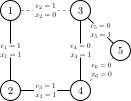
\includegraphics[width=\textwidth]{Chapter_V/BFS-example/a}
			\caption{}
			\label{fig:bfsExample:a}
		\end{subfigure}
		\hfill
		\begin{subfigure}[b]{0.22\textwidth}
			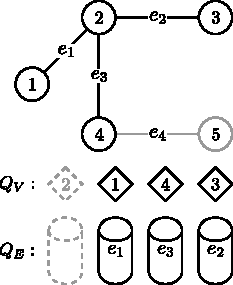
\includegraphics[width=\textwidth]{Chapter_V/BFS-example/b}
			\caption{}
			\label{fig:bfsExample:b}
		\end{subfigure}
		\hfill
		\begin{subfigure}[b]{0.22\textwidth}
			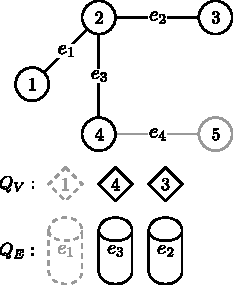
\includegraphics[width=\textwidth]{Chapter_V/BFS-example/c}
			\caption{}
			\label{fig:bfsExample:c}
		\end{subfigure}
		\hfill
		\begin{subfigure}[b]{0.22\textwidth}
			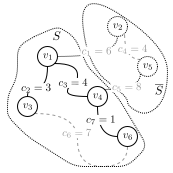
\includegraphics[width=\textwidth]{Chapter_V/BFS-example/d}
			\caption{}
			\label{fig:bfsExample:d}
		\end{subfigure}
		\hfill\null
		\caption[Kolejne kroki zmodyfikowanego algorytmu \textsc{BFS} $\left( T, v_{s}, v_{t} \right)$]{
			Kolejne kroki zmodyfikowanego algorytmu \textsc{BFS} $\left( T, v_{s}, v_{t} \right)$ (ang. \textit{Breadth-First Search}), gdzie $T$ jest drzewem rozpinającym graf $G$, $v_{s}$ oraz $v_{t}$ są odpowiednio wierzchołkami początkowym i~końcowym ścieżki $v_{s} \leadsto v_{t}$, dla której chcemy wyznaczyć zbiór krawędzi należących do $T$ i~do tej ścieżki.
			\textbf{(a)}~Początkowa sytuacja algorytmu dla $v_{s} = v_{2}$ i~$v_{t} = v_{5}$.
			Na koniec kolejki $Q_{V}$ został dodany wierzchołek początkowy.
			Odpowiadający mu element w~kolejce $V_{E}$ nie zawiera żadnych elementów.
			\textbf{(b)}~W wyniku zdjęcia z~kolejki pierwszego elementu $v_{2}$, algorytm dodał do $Q_{V}$ wszystkie wierzchołki, do których prowadziły krawędzie ze zdjętego wierzchołka.
			Odpowiednio dla każdego takiego wierzchołka, do kolejki $Q_{E}$ zostały dodane krawędzie, dzięki którym algorytm do nich dotarł.
			\textbf{(c)}~Zgodnie z~kolejnością ściągania elementów z~kolejek, aktualnie badanymi elementami (zaznaczonymi w~kolejce jasnym kolorem) są: wierzchołek $v_{1}$ oraz zbiór krawędzi $\left\{ e_{1} \right\}$.
			Z~tego wierzchołka nie prowadzi jednak żadna nowa krawędź, badany wierzchołek nie jest też tym końcowym, toteż algorytm usuwa wskazane elementy.
			\textbf{(d)}~W wyniku wykonania operacji na kolejnej parze elementów: $\left( v_{4}, \left\{ e_{3} \right\} \right)$, do kolejki priorytetowej $Q_{V}$ został dodany\footnote{
				Jako że dodawany wierzchołek jest wierzchołkiem końcowym ścieżki $v_{s} \leadsto v_{t}$, zamiast aktualizować obydwie kolejki, możemy odpowiadający mu (wierzchołkowi $v_{t}$) zbiór krawędzi od razu przenieść do puli znalezionych ścieżek bez modyfikacji kolejek i~przejść do następnego elementu.
			} nowy, jeszcze nieodwiedzony wierzchołek $v_{5} = v_{t}$.
			Równolegle, do kolejki $Q_{E}$ dla dodanego wierzchołka, został dodany zbiór krawędzi będący sumą zbioru łuków, po których algorytm dotarł do analizowanego wierzchołka $v_{4}$, oraz łuku, po którym przeszedł on do nowego wierzchołka (zbiór $\left\{ e_{3}, e_{4} \right\}$).
			Fakt, że dodawany do kolejki $Q_{V}$ element jest wierzchołkiem końcowym w~ścieżce $v_{s} \leadsto v_{t}$, oznacza, że podany zbiór krawędzi jest jedną z~możliwych ścieżek (w tym przypadku jedyną) pomiędzy tymi wierzchołkami.
			Algorytm kontynuujemy dopóki obie kolejki nie są puste, zapisując po drodze elementy z~$Q_{E}$, które odpowiadają wierzchołkom $v_{t}$, dodawanym do kolejki $Q_{V}$ (zapisujemy te ścieżki, których ostatnia krawędź prowadzi do $v_{t}$).
		}
		\label{fig:bfsExample}
	\end{figure}
\end{savenotes}



\subsection{Wady algorytmu zachłannego}



Jak każdy algorytm zachłanny, i~ten boryka się z~tymi samymi problemami: lokalny charakter jego decyzji powoduje, że bardzo łatwo zatrzymać mu się w~\textbf{lokalnym optimum} $T^{\left( \ast \right)}$, które charakteryzuje się tym, że dla dowolnego drzewa $T^{\prime} \in N \left( T, T^{\ast}_{\textbf{s}}, k \right)$ mamy $v_{\textsc{RRIMST}} \left( T^{\left( \ast \right)}, S \right) \leqslant v_{\textsc{RRIMST}} \left( T^{\prime}, S \right)$.
W~takiej sytuacji algorytm zachłanny oczywiście zakończy działanie z~przekonaniem, że znalezione przez niego rozwiązanie jest optymalne globalnie, choć w~rzeczywistości przeglądnięta przez niego przestrzeń rozwiązań dopuszczalnych była bardzo mała i~mogła ,,nie otrzeć'' się nawet o~prawidłowe rozwiązanie.
Oczywistą konsekwencją powyższego jest w~pełni deterministyczny schemat działania takiego algorytmu, tak więc jakość otrzymanego rozwiązania w~pełni zależy od zdanego przez nas początkowego drzewa $T^{\ast}_{\textbf{s}}$.
Dodatkowo algorytm nie uczy się~--- raz przeglądnięte przez niego rozwiązanie może być przeglądane dowolną liczbę razy, jeżeli zdarzy się, że dane rozwiązanie jest najlepsze w~sąsiedztwie wielu innych drzew rozpinających.
Jak zobaczymy w~części poświęconej algorytmowi lokalnego przeszukiwania z~listą ruchów zakazanych (ang. \textit{Tabu Search}), mimo tak licznych i~poważnych wad, algorytm ten jeszcze nam posłuży do konstrukcji dużo lepszego algorytmu.




\section{Symulowane wyżarzanie}




Algorytm \textbf{symulowanego wyżarzania} (ang. \textit{Simulated Annealing}) jest algorytmem mocno zbliżonym do poprzednio omawianego, jednak eliminuje pewne wady wspomnianego rozwiązania.
Przede wszystkim rezygnuje on z~przeglądania wszystkich sąsiadów zadanego drzewa $T$ (co wymuszało na nas wyrażenie $\min arg_{T^{\prime}} \left\{ v_{\textsc{RRIMST}} \left( T^{\prime}, S \right) \; : \; T^{\prime} \in N \left( T, T^{\ast}_{\textbf{s}}, k \right) \right\}$ w~linii $4$ pseudokodu \ref{alg:localsearch}).
Zamiast tego algorytm wprowadza pojęcie \textbf{temperatury}, która jest składową miary prawdopodobieństwa wybrania konkretnego sąsiada drzewa $T$ z~otoczenia $N \left( T, T^{\ast}_{\textbf{s}}, k \right)$.
Na jej podstawie, zamiast przeglądać całość otoczenia $N \left( T, T^{\ast}_{\textbf{s}}, k \right)$, algorytm losuje z~niego drzewo $T^{\prime}$, oblicza wartość takiego rozwiązania ($v_{\textsc{RRIMST}} \left( T^{\prime}, \textbf{s} \right)$) i na podstawie tej danej oraz temperatury decyduje się na wybór takiego drzewa, bądź losuje następne, do momentu, w~którym dla wylosowanego drzewa $T^{\prime}$ i~przekazanego do funkcji wyliczającej prawdopodobieństwo jego wybrania, zwrócona przez nią wartość jest dostatecznie wysoka.
Algorytm rozpoczyna pracę od pewnej temperatury maksymalnej, a~następnie ją sukcesywnie obniża, powodując spadek wartości obliczanych prawdopodobieństw~\cite{Nikulin2008}~\cite{Jany2015}.
Dodatkowo, w odróżnieniu od algorytmu zachłannego, każdy wykonany ruch pozwala na przeszukiwanie nowego otoczenia, zdefiniowanego jako $N \left( T, T^{\prime}, k \right)$, gdzie za $T^{\prime}$ przyjmujemy znalezione na chwilę obecną rozwiązanie, nie zaś jak to było do tej pory: $N \left( T, T^{\ast}_{\textbf{s}}, k \right)$.

Zaletami takiego rozwiązania w~porównaniu do poprzedniego algorytmu są niewątpliwie: brak konieczności przeglądania wszystkich sąsiednich rozwiązań (przeglądamy kolejne losowe rozwiązania do momentu, w~którym zdefiniowane wcześniej reguły pozwolą nam na wybranie jednego z~nich) oraz większa odporność na pozostanie w~obszarze lokalnego optimum (ze względu na wprowadzoną losowość wyboru następnego rozwiązania z~sąsiedztwa).
Nadal jednak taka szansa istnieje, dlatego skupimy się teraz na trzecim i~najbardziej złożonym rozwiązaniu, które w~zamian nie jest obarczone wadami poprzedników~--- algorytmem lokalnego przeszukiwania z~listą ruchów zakazanych.




\section{Przeszukiwanie z~listą Tabu}




Algorytm \textsc{\textbf{Tabu Search}}~\cite{TabuSearch} swoją nazwę zawdzięcza, wprowadzanemu przez siebie, dodatkowemu elementowi jakim jest \textbf{lista ruchów zakazanych} (ang. \textit{tabu list}).
Taką listą będziemy nazywać zbiór ruchów, których z~różnych względów bronimy algorytmowi wykonywać w~trakcie poszukiwania rozwiązania~--- w~ten sposób, jeżeli \textbf{kadencja} takiego elementu na liście \textit{tabu} będzie wystarczająco długa (przez pojęcie kadencji rozumiemy liczbę iteracji algorytmu jaką ten musi wykonać, aby mieć możliwość ponownego wyboru zakazanego ruchu), zapewnimy sobie brak wpadania przez algorytm w~cykle podczas poszukiwania rozwiązania\footnote{
	Analogicznie jak w~omawianym wcześniej, zmodyfikowanym algorytmie \textsc{BFS} $\left( T, v_{s}, v_{t} \right)$ (patrz rysunek \ref{fig:bfsExample}), tak w~przypadku algorytmu \textsc{Tabu Search} algorytm nie podejmie decyzji powtórzenia pewnych ruchów, gdyż będzie wiedział, że taki ruch już wykonał (można powiedzieć, że lista \textit{tabu} jest częściowym zapisem historii wykonywanych ruchów).
}.
Dodatkowo będziemy chcieli rozwiązać kwestię groźby trafienia i~pozostania w~lokalnym minimum~--- aby temu zapobiegać, będziemy co jakiś czas ,,resetować'' nasz algorytm, który w~takiej formie (upraszając) można przyrównać do wielokrotnego uruchamiania algorytmu zachłannego, za każdym razem dla innych drzew początkowych.
Przy tym wszystkim będziemy oczywiście chcieli, abyśmy, w~przypadku odnalezienia najlepszego rozwiązania do tej pory, mogli wykonać ruch do niego prowadzący, ignorując listę ruchów zakazanych.
O~rozwiązaniu, będącym efektem wykonania zabronionego ruchu, będziemy mówić, że spełniało ono \textbf{kryterium aspiracji}.

Aby zapewnić sobie przegląd jak największej przestrzeni rozwiązań dopuszczalnych problemu \textsc{IMST}, będziemy chcieli, aby każde następne drzewo, będące punktem wyjścia po ,,restarcie'' algorytmu, było jak najbardziej oddalone od drzew do tej pory przeanalizowanych.
Innymi słowy będziemy chcieli zaradzić kolejnej wadzie, którą wykazaliśmy przy okazji analizy algorytmu zachłannego~--- stosunkowo niewielkiego obszaru rozwiązań, które ten algorytm badał, zanim zatrzymywał się w~lokalnym optimum.
Dla algorytmu \textsc{Tabu Search} nie jest inaczej~--- podczas jednego pełnego przebiegu jesteśmy w~stanie przeanalizować niewielką tylko część dopuszczalnych rozwiązań, dlatego sztucznie będziemy wymuszać rozpoczynanie wyszukiwania rozwiązania od nowa, zaczynając szukać w~innych miejscach, tak jak to zaprezentowano w pseudokodzie \ref{alg:tabusearch}.
Tym samym rezygnujemy z idei przeglądania sąsiedztwa, definiowanego do tej pory jako $N \left( T, T^{\ast}_{\textbf{s}}, k \right)$~--- tak samo jak w przypadku symulowanego wyżarzania będziemy chcieli szukać rozwiązania niezależnie od wybranego punktu początkowego ($T^{\ast}_{\textbf{s}}$), z każdą iteracją algorytmu, w razie zajścia odpowiednich warunków, przyjmując nowe bazowe rozwiązanie $T^{\Delta\ast}$, dla którego następnie będziemy poruszać się w sąsiedztwie, określonym jako $N \left( T, T^{\Delta\ast}, k \right)$.



\subsection{Ocena ruchu}



Chcąc w~trakcie działania algorytmu wykonywać ruchy pomiędzy kolejnymi rozwiązaniami, musimy sobie odpowiedzieć na pytanie: jakie chcemy wybrać kryterium, które będzie decydowało o~tym, który ruch będziemy wybierali.
W~najprostszym przypadku, tak jak to ma miejsce w~algorytmie zachłannym, naszym kryterium jest po prostu funkcja $v_{\textsc{RRIMST}} \left( T, S \right)$, która zwraca wartość wyrażenia $v \left( T, \textbf{s} \right) + \max_{\textbf{s}^{\prime} \in S} \min_{T^{\prime} \in \mathcal{T}^{k}_{T}} v \left( T^{\prime}, \textbf{s}^{\prime} \right)$ dla konkretnego drzewa $T$.
Optymalnym ruchem w~tym przypadku nazwiemy taki wybór $T_{1} \in N \left( T, T^{\Delta\ast}, k \right)$, który zaowocuje najmniejszą wartością powyższego wyrażenia, gdzie jego wartość zależy tylko od wybieranego drzewa ($T^{\Delta\ast}$ to obecnie sugerowane przez algorytm rozwiązanie problemu \textsc{RRIMST}).
W~następnym rozdziale pokażemy (patrz wykresy \ref{fig:rrimst1}), że wybór tej strategii dla algorytmu \textsc{Tabu Search}, w~istocie nadaje mu zachowanie identyczne, co w~przypadku algorytmu zachłannego (taki też jego opis, bardzo uproszczony, przytoczyliśmy wcześniej).
Aby wykorzystać potencjał, drzemiący w~omawianym algorytmie, będziemy stosować inną funkcję, stanowiącą kryterium wyboru ruchów.
Niech dana będzie zatem funkcja $Mval \left( T, T_{1} \right)$, gdzie $T_{1} \in N \left( T, T^{\Delta\ast}, k \right)$, o~następującej definicji:

\begin{equation}\label{eq:moveValue}
	Mval \left( T, T_{1} \right) = \alpha_{1} \cdot \left( v_{\textsc{RRIMST}} \left( T, S \right) - v_{\textsc{RRIMST}} \left( T_{1}, S \right) \right) + \alpha_{2} \cdot \frac{\text{R} \left[ i, j \right]}{it} + \alpha_{3} \cdot \frac{\text{R} \left[ k, l \right]}{it} + \alpha_{4} \cdot \text{MR} \left[ i, j \right] + \alpha_{5} \cdot \text{MR} \left[ k, l \right]\text{,}
\end{equation}
gdzie jej kolejnymi elementami składowymi są:

\begin{itemize}
	\item $v_{\textsc{RRIMST}} \left( T, S \right) - v_{\textsc{RRIMST}} \left( T_{1}, S \right)$~--- wskaźnik poprawy wartości rozwiązania dla wybranego drzewa $T_{1}$ względem starej, liczonej dla drzewa $T$, z~którego szukamy najlepszego dla nas ruchu,
	\item $\text{R} \left[ i, j \right]$ oraz $\text{R} \left[ k, l \right]$ przechowują informacje na temat liczby wystąpień krawędzi $e_{ij}$ oraz $e_{kl}$ w~dotychczas wybieranych rozwiązaniach,
	\item $\text{MR} \left[ i, j \right]$ oraz $\text{MR} \left[ k, l \right]$ oznaczają odpowiednio średnie wartości funkcji $v_{\textsc{RRIMST}} \left( T_{ij}, S \right)$ oraz $v_{\textsc{RRIMST}} \left( T_{kl}, S \right)$, gdzie $T_{ij}$ oraz $T_{kl}$ oznaczają te wybrane wcześniej rozwiązania, w~których występuje krawędź $e_{ij}$ lub $e_{kl}$.
	Parametr $it$ wskazuje na numer aktualnej iteracji, zaś
	\item parametry $\alpha_{1}$, $\alpha_{2}$, $\alpha_{3}$, $\alpha_{4}$, $\alpha_{5}$ są dowolne i~mogą być eksperymentalnie zdeterminowane.
	Z~uwagi na fakt, że w~tak zdefiniowanej funkcji większe jej wartości odpowiadają lepszym wybieranym rozwiązaniom, wyszukanie najlepszego ruchu w~sąsiedztwie drzewa $T$ oznaczać będzie taki wybór $T_{1}$, dla którego wartość $Mval  \left( T, T_{1} \right)$ jest największa.
\end{itemize}

Widzimy, że tak zdefiniowana funkcja oceny ruchu daje nam dużo większe możliwości wpływania na rozwiązania: zależnie od dobranych parametrów możemy położyć większy nacisk na każdorazowe poprawianie wyników (gdy $\alpha_{1}$ jest odpowiednio duża w~stosunku do pozostałych parametrów), bądź inne właściwości dotychczasowych rozwiązań.
Jeśli zatem sprawą drugorzędną jest dla nas to, by wartość rozwiązania dla każdego następnego drzewa była lepsza ($v_{\textsc{RRIMST}} \left( T, S \right) - v_{\textsc{RRIMST}} \left( T_{1}, S \right) > 0$), manipulując odpowiednio parametrami $\alpha_{1}$, $\alpha_{2}$, $\alpha_{3}$, $\alpha_{4}$ czy $\alpha_{5}$, możemy albo położyć większy nacisk na częstotliwość pojawiania się danej krawędzi wchodzącej do rozwiązań (im częściej będzie się pojawiać, bądź tym lepsze średnie wartości dzięki niej będziemy otrzymywać, tym bardziej może nam się opłacać wybierać takie następne rozwiązania, które daną krawędź także zawierają), albo będącej z~nich usuwaną ($\alpha_{3}$, $\alpha_{5}$).
Z~drugiej strony zaś, jeżeli wartość $\alpha_{1}$ będzie na tyle znacząca, by mieć wpływ na całą wartość funkcji $Mval \left( T, T_{1} \right)$, ryzyko pozostania przez algorytm \textsc{Tabu Search} w~lokalnym optimum jest niewielkie (jeśli wartość $\alpha_{1}$ dominuje nad pozostałymi, wtedy~--- w~przypadku, gdy algorytm ,,utknął'' w~takim punkcie~--- wartości członu $\alpha_{1} \cdot \left( v_{\textsc{RRIMST}} \left( T, S \right) - v_{\textsc{RRIMST}} \left( T_{1}, S \right) \right)$ są bardzo małe, bądź można je przyrównać do zera\footnote{
	Poprzez zwrot ,,utknął'' mamy na myśli sytuację, w~której algorytm na przemian wykonuje powtarzające się ruchy, gdyż dla nich funkcja $v_{\textsc{RRIMST}} \left( \bullet, \bullet \right)$ zwraca najmniejsze wartości spośród całego otoczenia dla rozwiązań, pomiędzy którymi algorytm się cyklicznie porusza~--- jedynym ratunkiem w~takiej sytuacji byłoby ,,zresetowanie'' algorytmu.
}).
To właśnie tej funkcji oceny ruchu poświęcimy dłuższy fragment rozdziału, w~którym będziemy testować zachowanie się algorytmu dla różnych parametrów.



\subsection{Sąsiedztwo}



Analizując pseudokod \ref{alg:tabusearch}, nietrudno nie zauważyć, że w~linijce $9$ nagromadziliśmy bardzo dużą liczbę warunków~--- w~tym miejscu założyliśmy również, że skoro jesteśmy zainteresowani tylko takim sąsiadem $T^{\prime}$ drzewa $T$, dla którego wartość $Mval \left( T, T^{\prime} \right)$ jest największa spośród wszystkich wartości $Mval \left( T, T^{\prime\prime} \right)$ dla drzew $T^{\prime\prime} \in N \left( T, T^{\Delta\ast}, k \right)$, to nie potrzebujemy pamiętać jednocześnie pozostałych drzew w~sąsiedztwie\footnote{
	Tak jak na przykład pseudokod algorytmu \textsc{Tabu Search} w~\cite{Kasperski2012}, gdzie są rozdzielone kroki: wygenerowanie całego zbioru $N \left( T, T^{\Delta\ast}, k \right)$ oraz wybranie z~niego drzewa o~jak największej wartości funkcji oceny ruchu.
}.
W~naszym przypadku zatem drzewem $T_{N}$ jest drzewo które:

\begin{itemize}
	\item należy do bezpośredniego sąsiedztwa drzewa $T$ (różni się od niego dokładnie jedną krawędzią) oraz ma nie więcej niż $k$ krawędzi, które nie należą do drzewa początkowego $T^{\Delta\ast}$ (czyli $T_{N} \in N \left( T, T^{\Delta\ast}, k \right)$),
	\begin{itemize}
		\item ruch, polegający na przejściu od $T$ do innego dopuszczalnego rozwiązania $T^{\prime}$, nie znajduje się na liście \textsc{tabu} ($\left( i, j \right) \notin TABU$)\footnote{
			Poprzez parę elementów $\left( i, j \right)$ dla listy ruchów zakazanych będziemy wyrażać taki ruch, który w~wyniku usunięcia z~pierwszego drzewa $T$ krawędzi $e_{i}$ a~dodania $e_{j}$, przekształcił je w~drzewo $T^{\prime}$.
			To też będziemy mieli na myśli, posługując się zapisem na przykład takim: $T^{\prime} \notin TABU$~--- jeżeli rozwiązaniem, z~którego mamy decydować się na ruch jest $T$, powyższy zapis zabrania nam wykonania ruchu, polegającego na usunięciu krawędzi $e_{i}$ i~dodaniu $e_{j}$ takich, że $: T \setminus \left\{ e_{i} \right\} \cup \left\{ e_{j} \right\} = T^{\prime}$.
		},
		\item lub wartość rozwiązania problemu \textsc{RRIMST} dla drzewa $T^{\prime}$ jest lepsza (mniejsza) niż najmniejsza taka wartość znaleziona do tej pory (kryterium aspiracji~--- $v_{\textsc{RRIMST}} \left( T^{\prime}, S \right) < C^{\Delta\ast}$), 
	\end{itemize}
	\item $Mval \left( T, T^{\prime} \right)$ zwraca największą wartość spośród wszystkich drzew, które spełniają wszystkie powyższe kryteria ($T_{N} \leftarrow \max arg_{T^{\prime}} \left\{ Mval \left( T, T^{\prime} \right) \; : \dots \right\}$).
\end{itemize}

W przypadku, gdy zbiór $N \left( T, T^{\Delta\ast}, k \right)$ jest na tyle duży, że wykonanie powyższych obliczeń dla każdego drzewa należącego do tego zbioru w~sposób nieakceptowalny wpływa na czas wykonywania się algorytmu, możemy zastosować dodatkowo \textbf{kryterium aspiracji plus}, które przyjmuje parametry:

\begin{itemize}
	\item $min$~--- najmniejsza liczba drzew z~sąsiedztwa, które musimy przeglądnąć ($\min \left\{ min, \left| N \left( T, T^{\Delta\ast}, k \right) \right| \right\}$),
	\item $max$~--- liczba drzew ze zbioru $N \left( T, T^{\Delta\ast}, k \right)$, po których przeglądnięciu musimy zwrócić drzewo, dla którego wartość wyrażenia $Mval \left( T, \bullet \right)$ była największa do tej pory~--- reszty drzew rozpinających nie przeglądamy ($max = \min \left\{ max, \left| N \left( T, T^{\Delta\ast}, k \right) \right| \right\}$),
	\item $v_{min}$~--- próg aspiracji, po którego przekroczeniu przez wartość $Mval \left( T, \bullet \right)$ dla pierwszego drzewa ($T^{+}$ i~niech będzie ono $i$'tym przeglądanym drzewem) będziemy przeglądać jeszcze co najwyżej $q$ następnych w~kolejności sąsiadów drzewa $T$ ze zbioru $N \left( T, T^{\Delta\ast}, k \right)$, gdzie
	\item $q$ w~wyrażeniu $p = \min \left\{ i + q, max \right\}$ stanowi odgórnie narzuconą liczbę drzew do sprawdzenia (po znalezieniu $T^{+}$), zaś $p$ reprezentuje faktyczną ich liczbę, którą musimy jeszcze przejrzeć.
\end{itemize}

W takiej sytuacji, zamiast wykonywać obliczenia dla wszystkich drzew w~sąsiedztwie, przerywamy je w~chwili, gdy zajdą następujące warunki:

\begin{itemize}
	\item przeglądniemy $max$ drzew lub
	\begin{itemize}
		\item wartość funkcji $Mval \left( T, \bullet \right)$ dla pewnego drzewa $T^{+}$ jest większa bądź równa niż ustalony z~góry parametr $v_{min}$ oraz
		\item wykonamy potrzebne obliczenia jeszcze dla $p$ następnych drzew należących do $N \left( T, T^{\Delta\ast}, k \right)$.
	\end{itemize}
\end{itemize}

W tym przypadku zwróconym drzewem $T_{N}$ będzie albo najlepsze spośród pierwszych $max$ drzew, albo pierwsze takie drzewo ($T^{+}$), dla którego $Mval \left( T, \bullet \right) \geqslant v_{min}$, gdzie $v_{min}$ jest parametrem stosowanego kryterium aspiracji, albo najlepsze znalezione po nim ($T_{N} = \max arg_{T^{\prime}} \left\{ Mval \left( T, T^{\prime} \right) \; : T^{\prime} \in \left\{ T^{+}, T^{+2}, \dots, T^{+p} \right\} \right\}$).

\begin{pseudokod}[!h]
	\DontPrintSemicolon
	\SetKwInOut{Input}{Wejście}  
	\Input{
		$G = \left( V, E \right)$,\\
		$S$~--- zbiór scenariuszy adwersarza,\\
		$k$~--- parametr problemu \textsc{IMST},\\
		$it_{max}$~--- liczba iteracji, po której następuje ,,zresetowanie'' algorytmu.
	}
	\SetKwInOut{Result}{Wyjście}  
	\Result{
		$T^{\Delta\ast}$~--- najlepsze znalezione do tej pory rozwiązanie problemu \textsc{RRIMST}.
	}
	\Begin{
		$T \leftarrow \textsc{Random-MST} \left( G \right)$\tcp*{
			\parbox[t]{3in}{
				\raggedright Wybierz początkowe, losowe drzewo rozpinające graf $G$.
			}
		}
		$T^{\Delta\ast} \leftarrow T$\;
		$C^{\Delta\ast} \leftarrow v_{\textsc{RRIMST}} \left( T, S \right)$\;
		$TABU \leftarrow \emptyset$\;
		$E^{c} \leftarrow T^{c}$\;
		$it \leftarrow 0$\;
		\While{nie zaszło kryterium zatrzymania}{
			$T_{N} \leftarrow$ \small$\max arg_{T^{\prime}} \left\{ Mval \left( T, T^{\prime} \right) : T^{\prime} \in N \left( T, T^{\Delta\ast}, k \right) \; \wedge \;  \left( T^{\prime} \notin TABU \; \vee \; v_{\textsc{RRIMST}} \left( T^{\prime}, S \right) < C^{\Delta\ast} \right) \right\}$\;
			\normalsize$C_{N} \leftarrow v_{\textsc{RRIMST}} \left( T_{N}, S \right)$\;
			$it \leftarrow it + 1$\;
			\If{$C_{N} < C^{\Delta\ast}$\tcp*{
				\parbox[t]{3.8in}{
					\raggedright Znaleziono lepsze rozwiązanie.
				}}}{
				$T^{\Delta\ast} \leftarrow T_{N}$\;	
				$C^{\Delta\ast} \leftarrow C_{N}$\;
				$E^{c} \leftarrow E^{c} \cup T_{N}^{c}$\;	
				$it \leftarrow 0$\;
			}
			\uIf{$it > it_{max}$\tcp*{
				\parbox[t]{3.8in}{
					\raggedright Przekroczono liczbę iteracji.
				}}}{
				$T \leftarrow \textsc{Random-MST} \left( \left( V, E^{c} \right) \right)$\;
				$C \leftarrow v_{\textsc{RRIMST}} \left( T, S \right)$\;
				\If{$C < C^{\Delta\ast}$\tcp*{
					\parbox[t]{3.8in}{
						\raggedright Jeśli losowo wybrane, nowe początkowe drzewo rozpinające jest najlepsze.
					}}}{
					$T^{\Delta\ast} \leftarrow T$\;	
					$C^{\Delta\ast} \leftarrow C$\;	
				}	
				$TABU \leftarrow \emptyset$\tcp*{
					\parbox[t]{3.8in}{
						\raggedright Resetowanie algorytmu.
					}
				}
				$E^{c} \leftarrow T^{c}$\;
				$it \leftarrow 0$\;		
			}
			\Else{
				$T \leftarrow T_{N}$\;
				\textsc{Update-Tabu} $\left( \right)$\;
			}
		}
		\Return $T^{\Delta\ast}$\;
	}
	\caption{
		\textsc{Tabu-Search} $\left( G, S, k, it_{max} \right)$
	}
	\label{alg:tabusearch}
\end{pseudokod}



\subsection{Losowe drzewo rozpinające i~strategia dywersyfikacji}



Omawiając cele jakie chcemy zrealizować, implementując algorytm \textsc{Tabu Search}, wspomnieliśmy także o~chęci ,,resetowania'' algorytmu i~rozpoczynania jego pracy na nowo, lecz z~rozwiązaniem początkowym $T$ jak najdalej oddalonym od któregokolwiek drzewa, które pojawiło się w~procesie wykonywania się iteracji poprzedniej.
W~tym celu wprowadziliśmy następujące oznaczenia: $E^{c}$ oraz $T^{c}$, gdzie to pierwsze jest konstruowane z~sumy tych drugich.
$T^{c}$ będziemy nazywali \textbf{alternatywą najgorszego przypadku} dla drzewa $T$~--- innymi słowy będzie to minimalne drzewo rozpinające (znalezione przez zwykły algorytm rozwiązujący problem \textsc{MST}) dla scenariusza $\textbf{s}^{-} \left( T \right)$ o~następujących kosztach:

\begin{equation}
	c^{\textbf{s}^{-} \left( T \right)}_{i} = \left\{
	\begin{matrix}
		\max \left\{ c^{\textbf{s}}_{i} : \textbf{s} \in S \right\} & e_{i} \in T\text{,}\\ 
		\min \left\{ c^{\textbf{s}}_{i} : \textbf{s} \in S \right\} & e_{i} \notin T\text{,}
	\end{matrix}\right. 
	\qquad \forall i \in \left\{ 1, 2, \dots, m \right\}\text{.}
\end{equation}

Celem takiego zabiegu jest wymuszenie zwrócenia przez algorytm takiego minimalnego drzewa rozpinającego, którego część wspólna z~drzewem $T$ jest jak najmniejsza (które jest jak najbardziej oddalone od zbioru sąsiadów drzewa $T$~--- $\left\{ T^{\prime} \; : \; f \left( T^{\prime}, T \right) = 1 \right\}$).
Widzimy, że ilekroć poprawiamy dotychczas odnalezione rozwiązanie (poza sytuacją, w~której ,,resetujemy'' algorytm i~przez przypadek nowo wygenerowane drzewo okazuje się być tym najlepszym~--- linie $20$--$25$), do zbioru $E^{c}$ dołączamy krawędzie wygenerowanych alternatyw dla tych rozwiązań ($E^{c} \leftarrow E^{c} \cup T_{N}^{c}$).
Taka strategia skutkuje tym, że po $it_{max}$ iteracjach rozpoczynamy poszukiwanie rozwiązania w~zupełnie innym fragmencie przestrzeni rozwiązań dopuszczalnych, przez co mamy większą szansę ,,natknąć'' się na lokalne optimum, które jest również optymalne globalnie.

Generowanie losowych drzew rozpinających dany graf (linie $2$ oraz $20$) jest zadaniem prostym~--- w~tym przypadku również możemy skorzystać ze zmodyfikowanej wersji algorytmu \textsc{BFS}, bądź dowolnego innego, błądzącego po grafie w~sposób losowy (choć istnieją algorytmy od nich efektywniejsze~\cite{Wilson:1996:GRS:237814.237880}).
Najprostsza implementacja, wraz z~odwiedzaniem kolejnych krawędzi, po prostu losowo wybiera wychodzącą z~niego krawędź spośród dostępnych, dbając o~to, aby zakończyć ten proces w~chwili wybrania ostatniej, $\left( \left| V \right| - 1 \right)$'ej krawędzi (odwiedzając przy tym każdy wierzchołek tylko raz).



\subsection{Lista ruchów zakazanych i~kryterium końca}



Ostatnim elementem wymagającym omówienia jest lista \textsc{tabu}.
Dzięki niej jesteśmy w~stanie uniknąć zbyt częstego powtarzania tych samych ruchów czy wymusić na algorytmie przegląd coraz to dalszego sąsiedztwa danego drzewa początkowego w~kolejnych iteracjach.
Niestety, zastosowanie listy ruchów zakazanych ma swoje wady: fakt istnienia takiej listy może oznaczać, że w~pewnych sytuacjach najbardziej optymalny ruch jest zakazany i~nie będziemy mogli go wykonać (prawdopodobieństwo takiego zdarzenia jest tym większe im na dłuższe kadencje się zdecydujemy).
Przeciwdziałać takim przypadkom ma, wprowadzone przez nas, kryterium aspiracji, które w~sytuacjach takich jak opisana pozwala nam całkowicie zignorować listę \textsc{tabu}.
Wokół samego wyboru długości kadencji poszczególnych elementów listy gromadzi się wiele problemów; z~jednej strony powiedzieliśmy, że zbyt długie kadencje mogą powodować pomijanie pewnych optymalnych rozwiązań, lecz dzięki temu, że niektóre ruchy są zakazane przez bardzo długi okres, mamy szansę przeglądnąć szerszy obszar rozwiązań dopuszczalnych wokół punktu startowego.
Pociąga to za sobą również wady~--- przeszukując coraz to większy obszar przy niezmiennej liczbie iteracji, tracimy na jakości uzyskiwanych wyników (badany zbiór rozwiązań jest rzadszy, przez co większe jest prawdopodobieństwo pominięcia rozwiązania, które powinniśmy wybrać).
Z~kolei skłanianie się ku krótkim kadencjom podnosi co prawda naszą szansę na znalezienie optymalnego rozwiązania, lecz wraz z~nią rośnie zagrożenie, że zwróconym rozwiązaniem będzie optimum lokalne, bądź algorytm wpadnie w~cykl.

Z każdą następną iteracją, wraz z~wywołaniem procedury \textsc{Update-Tabu}, pozostały czas kadencji każdego z~elementów powinien ulec zmniejszeniu, zaś ruchy, których czas kadencji dobiegł końca~--- usunięte z~listy, co czyni je ponownie możliwymi do wyboru.
Dodatkowo, jako najprostsze kryterium końca algorytmu, możemy przyjąć warunek sprawdzający, czy całkowita liczba iteracji nie została przekroczona.
Jeżeli tak, zwrócimy najlepsze do tej pory odnalezione rozwiązanie.



\subsection{Podsumowanie rozdziału}



Algorytm \textsc{Tabu Search} jest tylko ideą~--- większa część pokazanego pseudokodu jest opcjonalna i~tylko od tego, do jakiego problemu się tę ideę zastosuje, zależy finalny kształt tego algorytmu.
Wszystkie podane parametry, takie jak okres kadencji, liczba iteracji, kryterium zatrzymania się algorytmu czy też parametry aspiracji plus, czy choćby poszczególne wskaźniki funkcji oceny ruchu (jak i~też sama funkcja)~--- powinny być rozpatrywane dla każdego problemu oddzielnie i~nie istnieje ogólna formuła wskazująca ich wartości.
W~przypadkach takich jak ten, którym się zajmujemy, gdy nie istnieje żaden algorytm wielomianowy, który zapewniałby nam zwracanie poprawnego rozwiązania (czy to optymalnego, czy gorszego od niego o~stały współczynnik), algorytm \textsc{Tabu Search} jest jednak bardzo dobrą alternatywą, o~której efektywności przekonamy się w~następnym rozdziale, testując działanie algorytmu dla różnych wartości jego parametrów, pokazując związki między nimi oraz analizując złożoności obliczeniowe problemów, które leżą u~podstaw zagadnienia \textsc{Recoverable Robust Incremental Minimum Sapnning Tree}.